\section{Introduction}
Ambient noise—particularly in the form of broadband sound such as white, pink, or brown noise—has been widely used for decades to aid in relaxation, concentration, and sleep. These noise types differ in their spectral properties: white noise contains equal energy per hertz across the entire frequency spectrum, pink noise emphasizes lower frequencies with equal energy per octave, and brown noise (also known as Brownian or red noise) further intensifies low-frequency components, creating a deeper, more soothing sound. Despite their widespread use, the process of selecting the optimal noise type and fine-tuning its characteristics—such as volume, spectral balance, and texture—is typically subjective, inconsistent, and labor-intensive.

Moreover, the human brain responds to auditory stimuli in highly individualized and context-dependent ways. A particular noise profile that enhances relaxation for one person may be ineffective or even distracting for another. Additionally, even within the same individual, the optimal auditory stimulus can vary depending on time of day, cognitive load, emotional state, and environmental context. Traditional static noise generators do not account for these dynamic physiological and psychological variables, resulting in suboptimal or inconsistent outcomes.

The Neuro-Adaptive NoiseScape system addresses these limitations by introducing a closed-loop, neurofeedback-based approach to noise generation. This system integrates real-time electroencephalography (EEG) monitoring with adaptive audio synthesis algorithms to create a responsive sound environment. By continuously analyzing the user’s brainwave activity—such as alpha (8–12 Hz), beta (13–30 Hz), and theta (4–7 Hz) rhythms, which are associated with different mental states—the system infers the user’s current level of relaxation or cognitive engagement. It then dynamically adjusts parameters of the noise being played, such as its spectral density, amplitude modulation, and frequency coloration, to promote the brain's progression toward a desired state (e.g., deep relaxation or sustained attention).

This neuroadaptive feedback loop transforms ambient noise from a static tool into an intelligent, responsive system that is both personalized and context-aware. By aligning auditory stimulation with real-time neural data, the Neuro-Adaptive NoiseScape provides a scientifically grounded and user-specific method for optimizing mental states, with potential applications in wellness, mental health, productivity, and sleep science.

\section{Theory}

An important foundation for understanding adaptive sound design lies in the neural correlates of mental states, as measured by electroencephalography (EEG). EEG captures brain activity in the form of electrical oscillations, which can be categorized into frequency bands that correlate with psychological states. For example, alpha waves (8–12 Hz) are associated with calm wakefulness, beta waves (13–30 Hz) with focused cognitive engagement, and theta waves (4–7 Hz) with drowsiness and meditative states \cite{klimesch1999}. By tracking these rhythms in real time, it becomes possible to infer an individual’s cognitive state and respond accordingly, laying the foundation for a neuroadaptive sound system.

This real-time responsiveness is grounded in the concept of closed-loop brain-computer interfaces (BCIs), which continuously sense neural activity and adapt stimuli to support or guide the brain toward a desired state. In a review by Sitaram et al. (2017), such closed-loop systems are shown to effectively enhance self-regulation, attention, and even clinical outcomes in disorders such as ADHD and depression \cite{sitaram2017}. Unlike open-loop systems, which act independently of user state, closed-loop designs enable dynamic and personalized adaptation—crucial for auditory environments aiming to optimize mental performance or rest.

A key mechanism through which sound can actively influence neural activity is auditory entrainment. Rhythmic auditory stimulation, such as binaural beats or amplitude-modulated tones, can synchronize neural oscillations with external rhythms. This synchronization has been shown to influence states of attention, relaxation, and sleep \cite{nozaradan2014}.

A significant contribution to the understanding of how auditory stimulation can modulate brain activity during sleep comes from Besedovsky et al. (2017). Their study employed a closed-loop auditory stimulation method synchronized with slow oscillations in the EEG to enhance deep sleep quality. The results demonstrated that such stimulation not only strengthened slow-wave sleep—a critical phase for physical restoration and memory consolidation—but also amplified markers related to the immune system's supportive functions \cite{besedovsky2017}. While their work primarily focuses on sleep physiology, it reinforces the broader concept that adaptive soundscapes can actively influence neural dynamics when coupled with real-time neurofeedback.

Another perspective is offered by stochastic resonance, a phenomenon in which a moderate level of noise can enhance the detection of weak neural signals. Söderlund et al. (2010) found that children with attention deficits performed better on memory tasks when white noise was introduced—highlighting that noise can act as a cognitive enhancer under specific neurological conditions \cite{soderlund2010}. This finding supports the hypothesis that adaptive noise, when matched to individual brain dynamics, could benefit cognitive functioning in both clinical and non-clinical populations.

Given the interindividual variability in auditory processing and neural response, personalization is not a luxury but a necessity in effective sound-based interventions. By leveraging machine learning techniques alongside EEG data, a noise generation system can be trained to detect and respond to subtle changes in the user’s state, adjusting spectral content, modulation, and texture to suit moment-to-moment needs.

Finally, the broader applications of neuroadaptive noise systems span domains such as productivity, mental health, education, and sleep science. As demonstrated in human-computer interaction research \cite{mark2016}, carefully tuned digital environments can reduce stress, enhance focus, and support cognitive recovery. A sound environment that adapts in real time to the brain’s needs could support deep work sessions, therapeutic interventions, or mindful rest in ways that static systems cannot.

Taken together, these theoretical foundations underscore the significance of integrating EEG-based feedback with adaptive audio systems. By doing so, ambient noise moves from being a passive background element to an intelligent, responsive tool for mental state optimization.




\section{Methodology}

This chapter outlines the methodological approach of the 	extit{NoiseScape} project, which aims to explore how different noise configurations affect the user’s mental state, specifically in terms of relaxation and focus. To achieve this, we developed a desktop application that integrates a brain-computer interface (BCI) device from OpenBCI and allows users to test various noise environments while recording their EEG data. The methodology combines principles from experimental psychology, neuroscience, and software engineering to create a structured system for data collection, analysis, and interpretation.

\subsection{Experimental Design}

The project was carried out in several iterative phases, beginning with the definition of project goals and technical requirements. The initial concept was to allow users to select a target mental state (relaxed or focused), expose them to different types of noise, and evaluate which configuration most effectively supports the desired state. The core metric for relaxation was defined as the power of alpha waves (8-12 Hz), commonly associated with calm and restful brain activity.

In the planning stage, we designed a structured experimental protocol. Each participant is guided through a series of tasks under controlled conditions. The relaxation task requires the user to close their eyes and relax or think about something calming for two minutes. This task is repeated under nine different auditory conditions: eight with different types and volumes of noise, and one silent baseline condition. The noise conditions include white, pink, brown, and green noise, each at two user-defined volume levels (low and high). These volume levels are not defined by precise decibels but by subjective user comfort, determined using sliders in the application interface.

\subsection{EEG Data Collection and Analysis}

EEG data is recorded using the OpenBCI headset and streamed via the 	exttt{openbci-python} library. The noise is generated using 	exttt{NumPy} and played back with the 	exttt{sounddevice} library. The EEG data is saved in labeled formats that correspond to the noise condition and task type. All data is stored in a structured directory path, which can be set by the user at the start of the experiment.

The data analysis is conducted offline. First, the EEG recordings are preprocessed using Python. Bandpass filtering (typically 0.5-50 Hz) is applied with 	exttt{SciPy} to remove noise outside the relevant EEG bands. Artifacts such as eye blinks may optionally be removed, though this step can be skipped for simplification. Alpha power is then calculated using spectral analysis methods like Fourier transforms or Welch’s method. The sum of power in the alpha band (8-12 Hz) is computed for each condition.

The main analytical goal is to compare alpha power across all conditions. By examining which noise condition results in the highest alpha power relative to the baseline, we can infer which noise setup best supports relaxation or focus. Trends in the data are visualized using bar plots, created with libraries such as 	exttt{Matplotlib}, showing the alpha power for each condition.






\section{Application}

\subsection{System Architecture and Technologies}

The development of \textit{NoiseScape} proceeded in parallel with the experimental design. Implemented as a cross-platform desktop application using \texttt{Electron} with a \texttt{Node.js} backend, the system is compatible with macOS and Windows, guiding users through the study in a structured and interactive way.

\begin{itemize}
\item \textbf{EEG Interface:} Real-time EEG data is streamed from an OpenBCI board via a Python backend using \texttt{openbci-python}, integrated into the application through a Node.js bridge.
\item \textbf{Noise Engine:} Broadband noise is generated using \texttt{NumPy}, spectrally shaped according to user-defined slider values, and played via the \texttt{sounddevice} library.
\item \textbf{Data Logging:} EEG recordings, along with the associated condition metadata (e.g. noise type and volume level), are stored in a user-selected, structured directory system.
\end{itemize}

\subsection{Graphical User Interface (GUI)}

The graphical user interface is divided into three vertical columns. The interface elements are numbered for clarity and to support referencing within figures.

\begin{figure*}[!t]
  \centering
  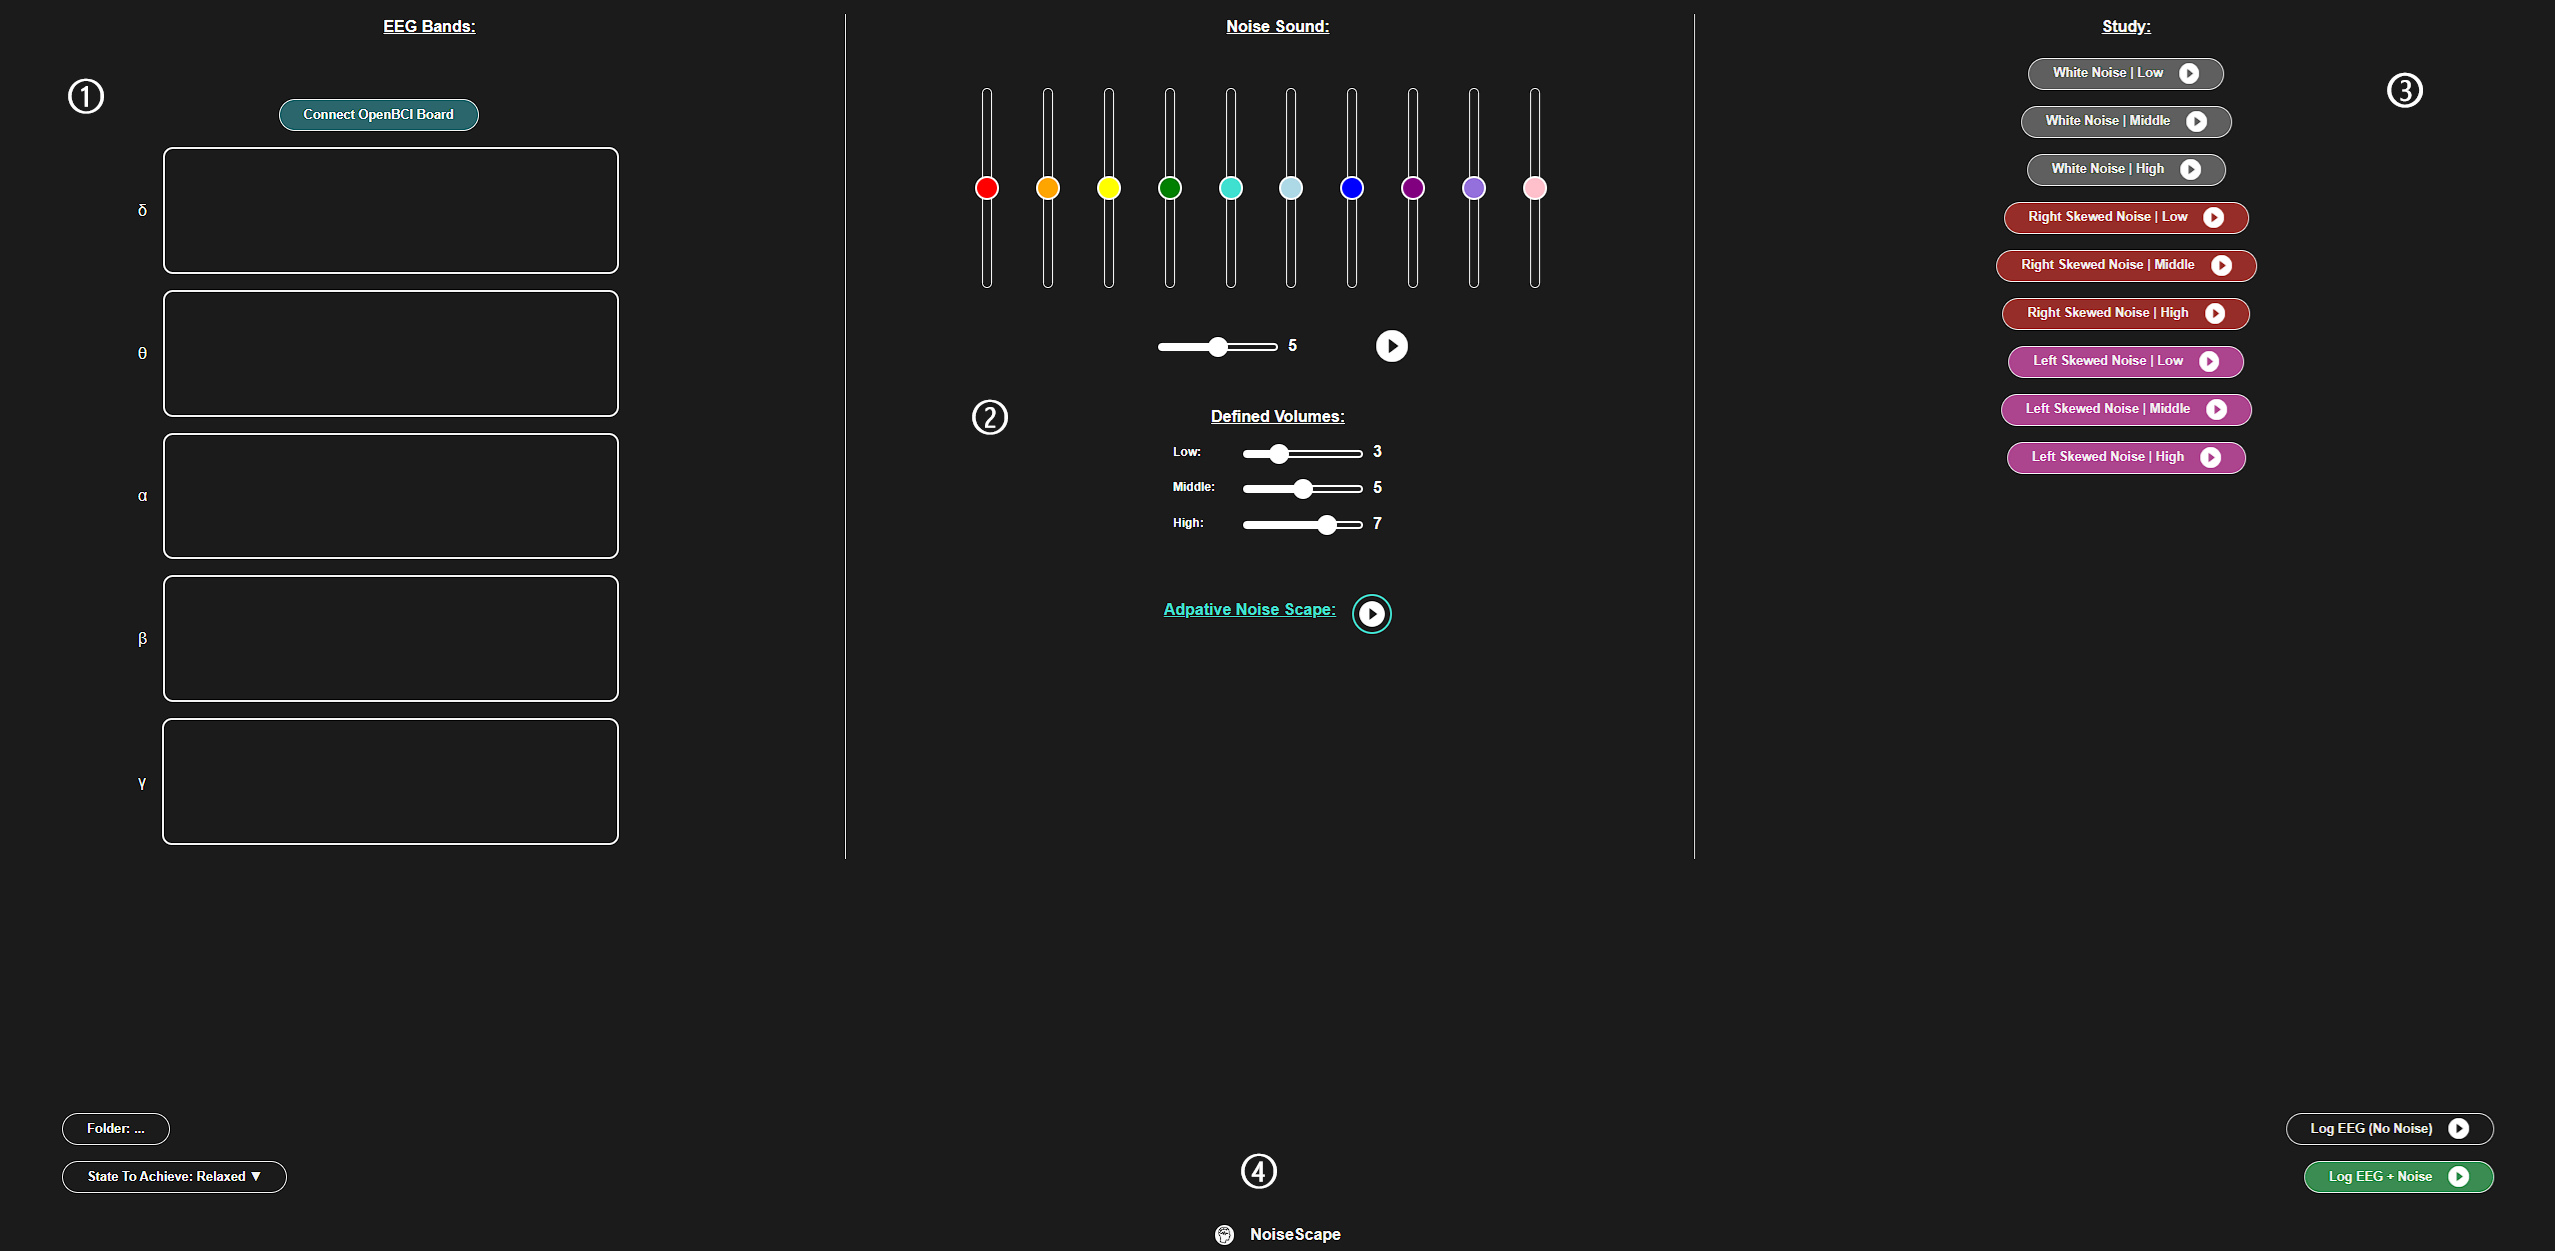
\includegraphics[width=\textwidth]{interface.png}
  \caption{Graphical user interface of the NoiseScape application.}
  \label{fig:interface}
\end{figure*}

\begin{enumerate}
\item \textbf{EEG Bands (Left Column)}

This panel displays real-time EEG power across five frequency bands: Delta ($\delta$), Theta ($\theta$), Alpha ($\alpha$), Beta ($\beta$), and Gamma ($\gamma$). Real-time EEG data is streamed from the connected OpenBCI device. A  button \texttt{`Connect OpenBCI Board'} initiates the device connection. \\

\item \textbf{Noise Sound – Free Play Mode (Center Column)}

This section allows manual control of noise spectrum playback through interactive elements:

\begin{enumerate}
  \item[(2a)] \textbf{Spectral Sliders (20 Hz–20 kHz):} Ten vertically arranged sliders are colored from left to right in rainbow hues. Each slider controls a specific frequency band of the white noise generator. When all sliders are centered (default), the full spectrum of white noise is played without weighting.

  \item[(2b)] \textbf{Playback Controls:} Below the sliders is a volume slider. To the right of this slider is a play button that toggles the current noise playback. When pressed, the noise corresponding to the current slider configuration is played at the defined volume level.

  \item[(2c)] \textbf{Defined Volumes:} Three additional horizontal sliders labeled \textit{Low}, \textit{Middle}, and \textit{High} are positioned below the main playback controls. These sliders allow the user to subjectively define what is perceived as low, medium, or high volume. They do not affect the actual playback volume but are referenced by the predefined study modes in the right column.

  \item[(2d)] \textbf{Adaptive Noise Scape:} Below the defined volume section is a button \textit{Adaptive Noise Scape}. This remains inactive until all nine study buttons (Section 3) and the baseline EEG condition (Section 4) have been completed and logged. Once enabled, it plays the noise configuration (as defined by the sliders and volume) that best matches the EEG patterns associated with the currently selected cognitive state (e.g., relaxed). \\
\end{enumerate}

\item \textbf{Study Mode (Right Column)}

The application supports three main types of spectral profiles, each derived from the same white noise base signal using the ten sliders:

\begin{itemize}
\item \textbf{White Noise:} All sliders are set to the middle position, resulting in a flat and unweighted frequency spectrum.
\item \textbf{Right-Skewed Noise:} Slider values decrease linearly from left to right , emphasizing low-frequency components.
\item \textbf{Left-Skewed Noise:} Slider values increase linearly from left to right, emphasizing high-frequency components.
\end{itemize}

Activating a study button sets the corresponding profile and enables logging of both the EEG data and the noise condition. The data is stored under structured filenames (e.g., \texttt{white\_low}, \texttt{left\_skewed\_middle}, \texttt{baseline}). \\

\item \textbf{Control Row (Bottom Section)}

The footer includes controls for file path selection, target state selection, and EEG recording.

\begin{itemize}
\item \textbf{Bottom Left:}
  \begin{itemize}
    \item \texttt{Set Root Path:} Opens a dialog allowing the user to select the root directory in which EEG data and metadata will be stored.
    \item \texttt{Select State to Achieve:} A dropdown menu \textit{State to Achieve}, currently limited to the value \textit{Relaxed}, allows the user to define the target state for adaptive noise optimization.
  \end{itemize}

\item \textbf{Bottom Right:}
  \begin{itemize}
    \item \texttt{Log EEG + NO Noise:} Starts a 2-minute EEG recording without any noise playback. This button is only active when no sound is currently playing. The resulting EEG data is saved under the label \texttt{baseline}.
    \item \texttt{Log EEG + Noise:} Starts a 2-minute EEG recording and logs both the EEG signal and the metadata of the currently playing noise condition. This button is only enabled if one of the nine study buttons is active.
  \end{itemize}
\end{itemize}

\end{enumerate}






\section{Discussion and Future Work}

The \textit{NoiseScape} system demonstrates the potential for using neuroadaptive feedback to customise ambient noise environments in real time. Integrating EEG data with dynamic sound synthesis enables nuanced, user-specific modulation of auditory stimuli, offering an alternative to traditional static soundscapes.

A central challenge observed during development was finding the right balance between system responsiveness and user stability. Real-time EEG data is inherently noisy and susceptible to artefacts (e.g. muscle movement or eye blinks), which can cause erratic fluctuations in noise modulation. Future iterations of the system could benefit from more robust signal pre-processing, possibly incorporating real-time artefact rejection algorithms or machine learning classifiers trained to detect stable mental states.

Another important for development is \textbf{longitudinal personalization}.  While the current version adapts to momentary brain states, a more intelligent system would learn a user’s patterns over time. By building a historical profile of EEG responses in different contexts (e.g. time of day, task type and emotional state), the system could proactively recommend or generate optimal noise configurations before cognitive fatigue or stress sets in. This could be achieved through online learning algorithms or reinforcement learning frameworks that continuously adjust audio parameters based on long-term reward signals, such as increased productivity or self-reported well-being.

One particularly promising application lies in \textbf{clinical contexts}, such as the treatment of anxiety, ADHD and insomnia. Neuroadaptive sound environments could complement or replace pharmacological interventions, offering an alternative with fewer side effects for cognitive regulation. For example, wearable EEG devices paired with mobile versions of \textbf{NoiseScape} could support daily functioning in children with attention deficit disorders and help patients with generalised anxiety disorder to engage in self-regulation exercises.

Furthermore, \textbf{integration with consumer devices} could drastically increase the system's scalability and accessibility. While these devices offer lower signal fidelity than research-grade EEG systems, this is sufficient for detecting significant changes in mental state. This could enable the continuous, passive adaptation of auditory environments during everyday activities, such as commuting, studying or sleeping.

Future development directions include:
\begin{itemize}
    \item \textbf{Multimodal feedback integration:} Combining EEG with physiological signals such as heart rate variability (HRV), galvanic skin response (GSR) or eye tracking.
    \item \textbf{Adaptive goal selection:} Supporting different cognitive states such as "focused", "relaxed" or "sleepy" via context-sensitive audio adaptation.
    \item \textbf{Real-time sonification of brain states:} Representing EEG activity directly through audio as part of biofeedback training.
    \item \textbf{Immersive VR/AR environments:} Embedding adaptive audio in virtual spaces to enhance presence, focus or therapeutic immersion.
    \item \textbf{Open data ecosystem:} Creating a shared dataset of EEG and noise condition mappings to encourage interdisciplinary collaboration.
\end{itemize}

Ultimately, the future of neuroadaptive sound systems lies in their ambient, universal integration — becoming a layer of cognitive support embedded in environments such as classrooms, offices, and therapeutic spaces.



\section{Conclusion}

The \textbf{NoiseScape} project demonstrates the potential of a new generation of intelligent auditory systems that can respond to the user’s mental state in real time. By leveraging EEG data to adapt the spectral properties and amplitude of broadband noise, the system transitions from being a passive sound generator to an active cognitive co-regulator. This personalised approach addresses the variability in how individuals respond to auditory stimuli and demonstrates the potential of closed-loop audio feedback in areas such as productivity and mental health.

Through its modular and extensible software framework, the project successfully combines the fields of neuroscience, audio engineering, and human-computer interaction. It provides a research platform for investigating EEG–sound interactions and lays the groundwork for further research or consumer applications. 

As the field of neurotechnology advances, systems like \textbf{NoiseScape} could become essential components of cognitive environments, optimising attention during work, deepening relaxation during meditation and enhancing therapeutic interventions in clinical settings. By synchronising digital auditory stimuli with brain rhythms, we are opening the door to a future where sound will support us as well as surround us.


%\begin{figure}\[h]
%\centering
%\fbox{\includegraphics\[width=0.7\linewidth]{figures/pilot\_results\_placeholder.png}}
%\caption{Example plot of alpha power across different noise conditions. (To be added after pilot data collection.)}
%\label{fig\:pilot\_results}
%\end{figure}